\section{The Emergence of Heterogeneous Computing}

    For several decades, from the 1970s until the early 2000s, advances in
    processor development followed Moore's Law \citep{4785860} and
    Dennard Scaling \citep{1050511}.
    This meant that the density of integrated circuits approximately doubled
    every two years, and processor clock frequencies increased proportionally
    while maintaining steady power consumption.
    This enabled continual processor improvements that were driven primarily by
    rising clock frequencies and microarchitectural refinements, enabling ever
    faster computations.

    The physics-driven nature \citep{Hutcheson2018Moore} of these advances in
    hardware has had important implications for software development.
    Not only did the performance of computers improve exponentially, but these
    performance gains were in the form of direct speedups, available to all the
    already existing programs.
    The primary interfaces between software and hardware - the instruction set
    architectures of processors - evolved gradually and with few
    paradigmatic changes \citep{8310168}.
    This is best exemplified by the pervasive x86 instruction set architecture,
    which still retains backward compatibility with its original inception in
    1978, and dominates desktop processors to this day.
    Software developers and users could, therefore, rely on ever-increasing
    performance from hardware progress alone, without any intervention.

\subsection{Via Multi-Processing to Heterogeneity}

    This continual progress started breaking down around 2005 with the apparent
    end of Dennard Scaling \citep{6307773}.
    While the shrinking of transistors continued, this no longer enabled
    proportionally increased clock frequencies with the same power budget.
    Processor designers instead started using the increasing transistor
    budget for adding additional processor cores.
    This shift toward multi-processing has left a deep mark on software
    development.
    New programming paradigms and languages, annotation systems, programming
    interfaces, libraries and compiler techniques were developed, and continue
    to evolve, to address the challenges of parallel computing.

    In recent years, transistor scaling has slowed significantly.
    In response to the now prevailing breakdown of both Dennard Scaling and
    Moore's Law, the hardware industry has turned toward architectural
    innovation \citep{7878935}.
    In particular, there is a trend toward specialised processor cores with
    that work in tandem as a heterogeneous system.
    Specialised processor cores outperform general-purpose cores on specific
    tasks.
    Furthermore, as heat dissipation has become a major challenge,
    simultaneously powering all transistors is often unviable, meaning that
    different processor cores have to be masked out dynamically at runtime
    (``dark silicon'') \citep{6307773}.
    Disabling a subset of a homogeneous multi-core system renders some of its
    cores redundant, whereas specialised cores can improve the system
    performance overall even if they are disabled most of the time and only
    used for the specific tasks at which they excel.

\section{The Diminished Role of Traditional Compilers}

    Heterogeneous computing can help overcome the scaling limitations of
    homogeneous, general-purpose processors.
    However, it also poses an enormous challenge to the associated software
    ecosystem, and it puts into question many of the achievements in portability
    and longevity of programs that are taken for granted in modern computing
    \citep{8719512}.
    Existing software does not automatically benefit from entirely new
    accelerator designs in the way that it profited from continuous
    improvements of established architectures.
    Where previously, programs performed better on each succeeding hardware
    generation, with at most a recompilation required, new accelerators arrive
    with novel and incompatible interfaces.

    In particular, this new hardware landscape greatly diminishes the scope of
    responsibilities and impact that traditional compilers for languages such as
    C, C++ and Fortran can have.
    Such compilers used to be responsible for orchestrating
    program execution on the entirety of available computing resources.
    They are now generally limited to only targeting the relatively small
    homogeneous fraction of processor cores directly.

\subsection{Libraries and Domain-Specific Languages}

    In order to reach peak performance on rapidly evolving and highly parallel
    hardware, novel programming models built around libraries and
    domain-specific languages have emerged.
    They succeed in utilising heterogeneous hardware in situations where
    traditional compilers fail.

    Two examples display the diversity of these approaches:
    Firstly, \citet{Ragan-Kelley2013Halide} developed the domain-specific
    language Halide for image processing.
    The Halide toolchain is able to generate fast code for heterogeneous
    platforms by focusing on a well-understood class of computations and by
    using a restrictive program representation.
    After tuning programs for particular platforms, it outperforms
    hand-optimised code, demonstrating an immense potential for domain-specific
    compiler optimisation under circumstances of constrained semantics.

    Secondly, Basic Linear Algebra Subprograms (BLAS)
    \citep{2002:USB:567806.567807}, a standard for library function interfaces
    going back to \citet{Lawson:1979:BLA:355841.355847} in the 1970s, have been
    implemented for most accelerators.
    These implementations are widely used and offer unrivalled performance.
    Some versions are provided directly by hardware vendors to support
    accelerators \citep{mkl,cublas,clblas,apl,qml}, while others originate as
    academic projects \citep{Wang:2013:AAG:2503210.2503219}.
    These different competing implementations use a plethora of approaches to achieve as
    close to peak performance as possible.
    This includes manually written assembly code, but also highly advanced
    code generation techniques, custom program representations and many more.

\subsection{The Consequences of Compiler Declining}

    Domain-specific languages and library interface make the full performance of
    heterogeneous systems accessible to programs.
    These success stories, however, leave significant problems unaddressed.
    The adoption costs are high, requiring application rewrites for
    accelerators.
    This coincides with often uncertain long-term prospects and minimal
    cross-platform portability.
    Even in the case of the agreed-upon BLAS standard -- arguably the best case
    scenario -- adoption of novel implementations is non-trivial in practice,
    due to the frequently encountered interface extensions for managing device
    handlers and memory synchronisation.
    For academic-backed domain-specific languages like Halide, on the other
    hand, complete rewrites are required in entirely novel software ecosystems,
    with an unclear future of support.

    On heterogeneous systems, programmers can rely on compilers for existing
    programming languages to evolve in lockstep with processor development.
    For example, even decades-old C++ source code compiles into efficient
    programs for the newest generation of x86 processors.
    Libraries and domain-specific languages are useful on homogeneous systems
    for achieving absolute maximum performance, but they become essential only
    in the context of heterogeneity.
    Therefore, the pervasive requirement for domain specific-languages and
    libraries only arises because compilers are unable to map programs onto
    specialised cores.
    Instead, compilers are increasingly downgraded to merely coordinating the
    launch of core workloads in the form of computational kernels, which are
    then executed as separate and opaque programs.

    It may appear evident that, for example, a full C++ or Java compiler cannot
    be provided for a typical graphics processor -- after all, most graphics
    processors have hardware limitations that prevent them from implementing the
    entire language standard.
    Indeed, many accelerators are even further from Turing complete.
    However, this should not prevent a partial compiler, offloading suitable
    subprograms, while falling back on homogeneous hardware providing a full
    language implementation for the remainder.
    After all, that is precisely the result achieved with libraries and
    domain-specific languages as well, and likely the desirable outcome.
    Despite the apparent convenience of such an approach, the next section gives
    reasons why this has not been championed so far.

\section{Host Compilers and Kernel Compilers}
\label{sec:hostkernel}

    While mainstream compilers for languages such as C/C++, Fortran or Java
    generally fail to exploit the full performance of heterogeneous systems, a
    specific class of compilers already play an essential role in
    targeting heterogeneous hardware.
    Many of the kernel programs that remain opaque to the application compilers
    are themselves products of other, specialised compilers.
    This necessitates a distinction between {\em host compilers} and {\em kernel
    compilers}.
    This distinction is mirrored by the differences between {\em host languages}
    and {\em kernel languages}.
    Host compilers translate full programs written in host languages,
    such as the previously mentioned C/C++, Fortran and Java, while kernel
    compilers handle small computational kernels that are expressed in dedicated
    domain-specific programming languages.
    The two classes of compilers have developed distinctly.
    Kernel compilers successfully apply many of the techniques that are severely
    limited on host compilers
    \citep{Murphy2014LimitsOD,Maleki:2011:EVC:2120965.2121464}.
    They reason automatically about parallelism
    \citep{Steuwer:2017:LFD:3049832.3049841}, have more sophisticated models to
    track data dependencies \citep{Baghdadi:2019:TPC:3314872.3314896}, and they
    incorporate iterative compilation techniques
    \citep{Ansel:2014:OEF:2628071.2628092}.

    This is made possible by a combination of factors that apply uniquely to
    kernel compilers:
    Smaller programs allow for more expensive compilation techniques;
    more restrictive languages and intermediate representations allow for
    stronger reasoning;
    abstractions in kernel compilers can be customised for the exact hardware
    architecture of accelerators;
    and domain knowledge from areas such as image processing can be directly
    embedded in custom compiler technology, without requiring their validity
    on generic programs.
    Furthermore, kernel compilers often run in more controlled environments,
    with less need for predictability, reproducibility, and stability.
    The range of input programs might even be small enough to ship them in
    already compiled form, making the compiler merely a tool in a
    library-implementation process.

    As host compilers operate under less forgiving conditions, it is
    unsurprising that they have lagged behind these developments.
    Because they cannot rely on such a restricted environment, host compilers
    are unable to match the optimisation capabilities of kernel compilers.
    Domain specific compilers and languages, as well as libraries, have
    therefore not been championed only because their restricted program
    spaces match the capabilities of particular heterogeneous accelerators.
    The restricted environment also makes them intrinsically more powerful and
    able to generate better code.

    Hybrid approaches, such as OpenCL, reinforce these observations.
    The language is domain specific only in its expression of parallelism, but
    otherwise designed to be general purpose.
    Compilers are provided for many structurally different processors.
    However, as a consequence of being a relatively unrestricted language, the
    compilers often underperform and the language is notoriously lacking in
    performance portability \citep{Falch:2015:MLB:2863697.2864570}.
    Partial compilers that require the same compromises as OpenCL -- being
    unable to utilise the restricted nature of input programs -- would surely
    suffer the same shortcomings.

\subsection{The Spectrum of Specialisation}

    General-purpose programming languages, domain-specific languages and
    accelerator libraries exist on a spectrum of specialisation.
    \Cref{specialgradient} provides some intuition about this spectrum by
    plotting popular languages and compute libraries onto their
    potential position.
    On the far left are versatile general-purpose languages, such as
    C/C++ and Fortran.
    Moving right, flexibility is gradually lost, with BLAS libraries at
    the end providing only fixed-function computations.
    At the same time, however, the restricted semantics allow for increased 
    optimisation capabilities.

    It is necessary to clarify what is meant by optimisation potential in this
    context and how it differs from raw performance.
    C/C++ is, of course, very suitable for manual optimisation and renowned as a
    low-overhead, high-performance language.
    However, it is difficult for compilers to apply deep structural changes to
    C/C++ programs correctly.
    Maintaining the semantics of BLAS routines, on the other hand, is viable
    with many structurally different implementation approaches.
    Therefore, C/C++ is fast because of its low overhead, and because
    programmers write efficient programs to begin with.
    By contrast, BLAS is fast because its semantics are so constrained that
    implementations can be tuned to perfection.

\begin{figure}[t]
\centering
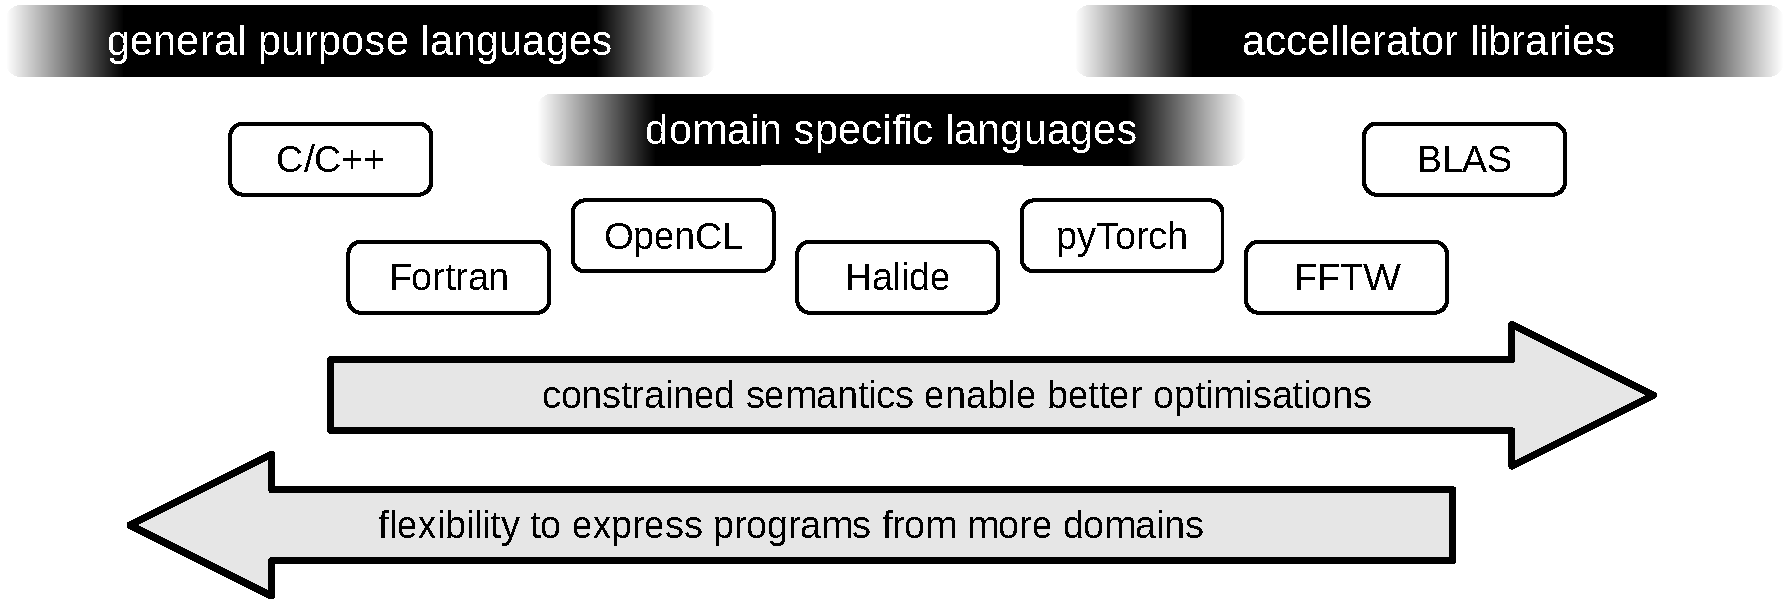
\includegraphics[width=\textwidth]{figures/DSLgradient}
\caption{Domain specific languages on a spectrum between general purpose
         languages and libraries.
         Decreasing flexibility allows for stronger reasoning and greater
         optimisation potential.}
\label{specialgradient}
\end{figure}

    In conclusion, the superior optimisation potential of libraries and
    domain-specific kernel compilers is a consequence of operating in more
    constrained conditions than host compilers.
    While expert programmers can often apply domain knowledge themselves
    when using versatile general-purpose languages, this potential can be
    automatically uncovered by specialised tools.
    The restrictions on input programs imply domain knowledge that is leveraged
    to make stronger assumptions, use more powerful models and generate better
    code.

    {\bf
    More restrictive program models result in additional optimisation
    opportunities and increased portability.
    Compilers use program models that correspond closely to their input
    programming languages.
    This correspondence could be decoupled by automatically recognising program
    parts that adhere to more constrained models, making the powerful
    domain-specific optimisation techniques of kernel compilers available to
    host compilers.
    }

\section{Moving on the Spectrum of Specialisation}

    To combine the positive aspects of both sides of the spectrum of
    specialisation, host compilers need methods to recognise more restrictive
    programming models within general-purpose code automatically.
    Reformulating the adhering program sections in domain-specific
    representations then makes the superior domain-specific reasoning from
    kernel compilers applicable also in the host compiler.

    Such an approach of detecting restricted models in general-purpose code has
    previously been used only for specific individual domains, and this involved
    extensive hand-implemented compiler analysis functionality.
    For example, the Polly compiler by \citet{Lengauer2012Polly} takes as
    input arbitrary C/C++ code and then recognises whether parts of this code
    are expressible in the more restrictive polyhedral model
    \citep{Karp:1967:OCU:321406.321418,benabderrahmane2010polyhedral}.
    The compiler then reformulates the relevant code in this system, which
    makes advanced optimisation techniques applicable that use the available
    domain knowledge of the restricted model for generating faster code
    \citep{Moll:2016:ISS:2892208.2892217,Doerfert2015Polly}, substantiating the
    hypotheses of \Cref{sec:hostkernel}.

\subsection{Contributions of this Thesis}

    This thesis derives a systematic approach for recognising constrained
    program sections during the compilation process that is not restricted to a
    particular model.
    The approach emerges from the analysis of a standard program model that host
    compilers use: Static Single Assignment (SSA) form intermediate
    representations.
    These SSA form representations are accessible to mathematical reasoning,
    with their most relevant features based on graph and list structures.
    With this in mind, structural restrictions on intermediate representation
    code -- corresponding to restricted, domain-specific models -- can be
    precisely formulated as mathematical constraints on a model of SSA form
    representations.
    The use of constraint solver techniques then makes automatic detection of
    adhering code regions feasible.

    Instead of manually implementing compiler analysis passes to recognise
    restricted models, a flexible constraint programming language is introduced,
    that can express many different such domain-specific models, and an
    accompanying toolchain is developed that uses these specifications to
    detect code sections that satisfy them automatically.
    This system captures the spectrum from \Cref{specialgradient}.
    On one extreme, sections of code are recognised as implementing
    specific algorithms, like matrix multiplications, that are merely
    parametrised with numbers.
    Next are algorithms that allow parametrisation with an operator.
    Stencil kernels, reduction operations or generalised histogram computations
    fall into this category.
    More generic again are programs that merely follow specific structural
    restrictions, such as code adhering to the polyhedral model.
    \Cref{chapter:candl,chapter:reductions,chapter:idioms} cover each of these
    domains, culminating if a system for the automatic heterogeneous
    acceleration of idiomatic code.

\section{Summary}

    The end of Moore's Law and Dennard Scaling has resulted in a shift away from
    homogeneous multi-processing, toward architectural innovation and
    specialised processor cores.
    The rising heterogeneity of computing resources poses a challenge to
    established compiler toolchains, which often only access the increasingly
    marginal homogeneous fraction of processing power.
    Therefore, programmers depend on domain-specific languages and libraries,
    which leverage domain knowledge from their restricted operating domains, to
    generate efficient code for this new hardware landscape.

    This domain knowledge can be made available to host compilers with
    approaches that automatically specialise general-purpose code and
    reformulate it in more restrictive program models.
    Previous work has established this on individual models, but this thesis
    develops a framework to formulate a wide range of restricted program models
    using a systematic approach based on constraints.
    To this purpose, a custom constraint programming language is introduced
    and successively extended.
    Starting from a discussion of the underlying assumptions and features of
    Single Static Assignment code, the methodology is developed into a complete
    system, implemented as part of the mature Clang C/C++ compiler.

    In the later chapters, this core system is then applied in combination
    with other techniques in a range of different contexts.
    This includes the rapid prototyping of compiler optimisations, the
    automatic parallelisation of some program structures with indirect memory
    accesses, a new formulation of the polyhedral model and the detection of
    computational structures that cover important bottlenecks in typical
    scientific programs.

    Eventually, the techniques are combined into a fully integrated, extensible
    compiler tool for efficiently mapping sequential programs onto heterogeneous
    systems.
    This develops the thesis all the way from abstract discussions of
    constraint programming approaches in compilers to the evaluation of real
    performance improvements on established benchmark suites and scientific
    applications.
    \vfill

%    \subsection*{extra building blocks}



%    The thesis develops a methodology to generalize this approach, resulting in
%    methods by which compilers can automatically classify code as adhering to
%    additional semantic constraints beyond what is guaranteed by the programming
%    language.
%    Using this classification, the compiler can then translate the code into a
%    more specialized domain and apply the already developed domain specific
%    techniques -- in the simplest case by merely linking to a library -- to
%    achieve full performance.


%    The implication of this is that in order to achieve best performance, it is
%    generally advisable to choose the most specialised tools available.
%    However, considerations of portability and maintainability push programmers
%    in the opposite direction, towards a small number of well established host
%    compilers and traditional languages at the expense of performance.



%    What is promising therefore is a combination of hand-optimised libraries,
%    domain specific languages together with compiler automatisms.
%    This requires a disruptive improvement in compiler analysis capabilites.
%    The detection of higher level algorithmic structures in compilers has been
%    investigated before, but established approaches cannot scale to what
%    this challenge requires.
%    Syntactic matching directly on programming languages has become
%    unviable for the complexities of both modern programming languages and
%    complex code bases.

%    Instead, this thesis develops an entirely novel approach based on concepts
%    from constraint solving, building a pragmatic methodology for detecting
%    complex algorithmic structures -- computational idioms.

%    In order to successfully target heterogeneous systems, host compilers need
%    to leverage the know-how that already exists in the surrounding software
%    ecosystem, encapsulated in special purpose libraries and code generators.

%    A linear alebra compiler operates under the assumption that the program is
%    linear algbera, and the program representation that is used with not even
%    allow the expression of any other system.

\pagebreak

\section{Structure of the Thesis}

    This thesis is divided into six chapters.
    Following the introduction, the underlying methodology of this work is
    established in {\bf\Cref{chapter:theory}} and put in the context of
    conventional compiler analysis.
    Based on a mathematical model of Static Single Assignment (SSA) form
    compiler intermediate representations, the chapter derives a novel
    constraint programming approach to express algorithmic program
    structures as constraint formulas.
    Finally, the chapter discusses implementation decisions,
    algorithmic complexity, and the relation to established Satisfiability
    Modulo Theory (SMT) problems.
    This forms the methodological basis for
    {\bf\Cref{chapter:candl,chapter:idioms,chapter:reductions}}.

    {\bf\Cref{chapter:literature}} gives a broad overview of the related work.
    This literature survey covers the four main areas of research in which this
    work is placed.
    Firstly, {\em constraint programming} underpins the methodology of this
    thesis.
    Secondly, {\em compiler analysis and auto-parallelisation} provide
    competing approaches against which the results in this thesis are evaluated.
    Thirdly, {\em heterogeneous computing} and the corresponding challenges
    motivate many of the compiler approaches that this research implements.
    Finally, ``{\em computational idioms}'' is an umbrella term for several
    overlapping concepts of algorithmic patterns that capture programming models
    in different positions on the spectrum of specialisation.

    {\bf\Cref{chapter:candl,chapter:idioms,chapter:reductions}}
    are each based on a published research article and elaborate on different
    applications of constraint programming in compilers.

    {\bf\Cref{chapter:candl}} develops a full-fledged constraint programming
    language called CAnDL, with an implementation in the LLVM compiler,
    infrastructure that automatically generates compiler analysis passes from
    declarative specifications.
    The chapter explores several compiler analysis challenges using CAnDL,
    including the rapid implementation of peephole optimisations and the
    prototyping of graphics shader optimisations.
    The chapter is based on published research in
    \citet{Ginsbach:2018:CDS:3178372.3179515}.

    {\bf\Cref{chapter:reductions}} develops an auto-parallelising compiler for
    complex reduction and histogram computations using CAnDL-powered analysis
    functionality.
    This covers many computations that are inaccessible to established
    approaches based on data flow and polyhedral analysis due to indirect memory
    accesses, demonstrating the greater flexibility of constraint programming.
    The chapter is based on published research in
    \citet{ginsbach2017discovery}.

    {\bf\Cref{chapter:idioms}} extends CAnDL into the Idiom Description Language
    (IDL) and applies it for detecting algorithmic structures that go beyond the
    scope of traditional compiler analysis: stencil computations, complex
    reductions and histograms as well as sparse and dense linear algebra.
    The resulting detection passes in LLVM enable automatic heterogeneous
    acceleration of sequential code and result in significant speedups on
    established benchmark suites.
    The chapter is based on published research in
    \citet{Ginsbach:2018:AML:3173162.3173182}.

\newpage
\phantom{placeholder}
\newpage